\section{Auswertung}
\label{sec:Auswertung}

%Im folgenden werden die Mittelwerte mit
%\begin{equation}
%  \label{eqn:mittelwert}
%  \bar x = \frac 1n \sum_i^n x_i
%\end{equation}
%und die Standardabweichung mit
%\begin{equation}
%  \label{eqn:stdabweichung}
%  \Delta\bar x = \frac{1}{n(n-1)}\sum_i^n (x_i- \bar x)^2
%\end{equation}
%berechnet.
%Aus Werten mit Unsicherheiten lassen sich mithilfe der Gauß'schen Fehlerfortpflanzung, die daraus abgeleiteten Größen berechnen, die
%folgendermaßen definiert ist:
%\begin{equation}
%  \label{eqn:gauß}
%  \Delta f= \sqrt{\sum_i^n \Big(\frac{\partial f}{\partial x_i}\cdot x_i \Big)^2}
%\end{equation}


\subsection{Apparatekonstante}
\label{sec:Apparatekonstante}
%Die Berechnung der Winkelrichtgröße $D$ berechnet sich über \autoref{eqn:winkelrichtgr} mit dem konstanten Abstand 
%$a= 10\si{\centi\meter}$ zu den folgenden Werten.
Aus \autoref{tab:winkelrichtgroesse} lassen sich die Messwerte der Kraft $F$ unter der Auslenkung $\varphi$ entnehmen, woraus sich die
Winkelrichtgröße $D$ über \autoref{eqn:winkelrichtgr} mit dem konstanten Abstand $a=\SI{10}{\centi\meter}$ berechnet.


\begin{table}[H]
  \centering
  \caption{Winkelrichtgröße $D$.}
  \label{tab:winkelrichtgroesse}
  \begin{tabular}{c c c}
      \toprule
      Auslenkung $ \varphi \;/\; \text{DEG}$ & $F \;/\; \si{\newton}$ & $D \;/\; \si{\newton\meter}$\\
      \midrule
      70 & 0.20 & 0,01637 \\
      80 & 0,24 & 0,01719 \\
      90 & 0,28 & 0,01783 \\
      100 & 0,33 & 0,01891 \\
      110 & 0,35 & 0,01823 \\
      120 & 0,39 & 0,01862 \\ 
      130 & 0,41 & 0,01807 \\
      140 & 0,47 & 0,01924 \\
      150 & 0,49 & 0,01872 \\
      160 & 0,52 & 0,01862 \\
      170 & 0,55 & 0,01854 \\
      \bottomrule
  \end{tabular}
\end{table}

%Woraus sich der Mittelwert für die Winkelrichtgröße ergibt.
Es ergebibt sich der Mittelwert für die Winkelrichtgröße zu
\begin{equation}
  \overline D = (0,01821\pm 0,0008274) \si{\newton\meter}.
\end{equation}
Das Trägheitsmoment der Drillachse ergibt sich mit zwei Gewichten.
Sie haben ein zylinderförmiges Gewicht von $m_1 = (223.2 \,\pm 0.1) \text{g}$ und $m_2 = (222.8 \,\pm 0.1)\, \text{g}$ und jeweils eine
Höhe $h=\SI{30}{\milli\meter}$ und einen Durchmesser $d=\SI{35}{\milli\meter}$.
\autoref{tab:eigentraegheitmess} sind die Messwerte der Schwingungsdauer der beiden Gewichte $T$ unter einem Abstand $a$ zu entnehmen.

\begin{table}[H]
  \centering
   \caption{Messwerte zum Eigenträgheitsmoment $I_D$.}
   \label{tab:eigentraegheitmess}
   \begin{tabular}{c c}
       \toprule
       Schwingungsdauer $ T \;/\; \si{\second}$ & Abstand $a \;/\; \si{\milli\meter}$ \\
       \midrule
       3,08 & 60 \\
       3,40 & 80 \\
       4,32 & 100 \\
       4,83 & 120 \\
       4,32 & 140 \\
       4,83 & 160 \\
       5,37 & 180 \\
       5,76 & 200 \\
       6,28 & 220 \\
       7,36 & 240 \\
       \bottomrule
   \end{tabular}
\end{table}


%Die Trägheitsmomente der beiden Gewichte lassen sich mithilfe (\autoref{eqn:steiner}) vereinfachen zu 
%\begin{equation}
%  I_1 = I_{\text{Zylinder}} + m_1a^2 = 1\si{\kilogram\meter^2}
%\end{equation}
%\begin{equation}
%  I_2 = I_{\text{Zylinder}} + m_2a^2 = 1\si{\kilogram\meter^2}
%\end{equation}


%Trägheitsmomente der Drillachse wird mit linearer Regression berechnet.

\sloppy
Die Trägheitsmomente der beiden Gewichte lassen sich mithilfe \autoref{eqn:steiner} vereinfachen. Zur Berechnung
des Trägheitsmomentes der Drillachse $I_D$, wird eine lineare Regression der Form
\begin{equation}
  \label{eqn:linReg}
  T^2 = ba^2+c
\end{equation}
verwendet.
Die Messwerte und die Regression sind in \autoref{fig:Plot} aufgetragen. Die Trägheitsmomente werden mit 
(\ref{eqn:Istab}) und (\ref{eqn:Izylinder}) berechnet (\cite{Anleitung}).
Die abgebildete lineare Regression der Form $ y = ax + b \,$ liefert die folgenden Werte
\begin{center}
  $ a = 0,828 \pm 0,008254 \frac{\si{\s^2}}{\si{\m^2}}$, \\
  $ b = 6,648 \pm 0,2572 \si{\s^2}$. \\
\end{center}

\begin{figure}[H]
  \centering
  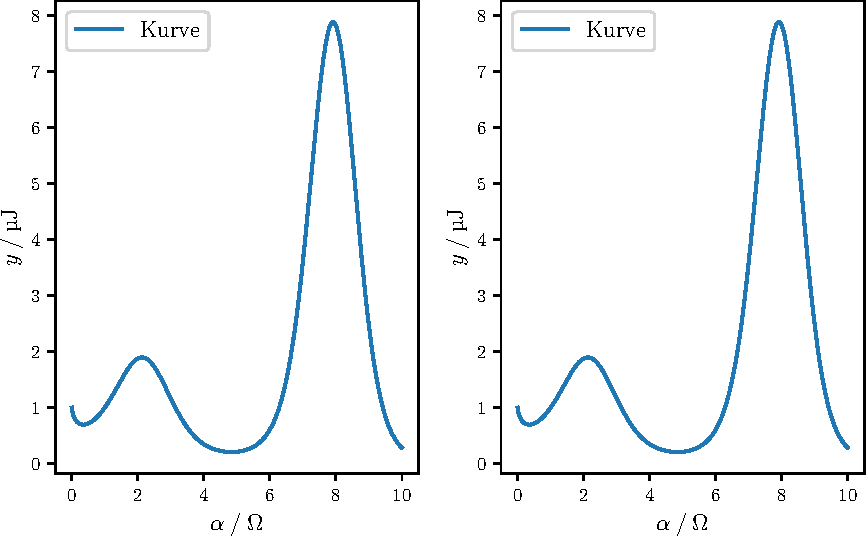
\includegraphics{plot.pdf}
  \caption{Messwerte und lineare Regression}
  \label{fig:Plot}
\end{figure}
Daraus folgt für das Trägheitsmomentes der Drillachse mit
\begin{equation*}
  I_D = \frac{bD}{4 \pi ^2} - 2m (\frac{r^2}{4} + \frac{h^2}{12})
\end{equation*}
und
\begin{equation*}
  \Delta I_D = \sqrt{(\frac{b}{4 \pi ^2})^2  (\Delta D)^2 + (\frac{D}{4 \pi ^2})^2  (\Delta b)^2}
\end{equation*}
der Wert $I_D = (2,999 \pm 0,1830) \cdot 10^{-3} \si{\kilogram\meter^2}$.

\subsection{Trägheitsmomente einfacher Körper}
\label{sec:Trägheitsmomente einfacher Körper}

Untersucht werden ein Zylinder und eine Kugel, dessen Rotationsachse je die Schwerpunktsachse der beiden Körper ist.
Die Trägheitsmomente des Zylinders und das der Kugel berechnen sich nach \autoref{fig:traegheitsbsp}.

%\begin{equation}
%  I_{\text{Zylinder}} = \frac{1}{2} mR^2
%\end{equation}



%\begin{equation}
%  I_{\text{Kugel}} = \frac{2}{5} mR^2 \, .
%\end{equation}

\sloppy Die Werte der beiden Körper sind
\begin{align*}
  m_{\text{Kugel}} &= (810,9 \pm 0,1)\:\si{\gram}, \\
  d_{\text{Kugel}} &= \SI{12,7}{\centi\meter}, \\
  m_{\text{Zylinder}} &= (367,8\pm 0,1)\:\si{\gram}, \\
  d_{\text{Zylinder}} &=  \SI{8,72}{\centi\meter}, \\
  h &= \SI{9,00}{\centi\meter}. \\
\end{align*}
Damit ergeben sich die Theoriewerte der Trägheitsmomente für den Zylinder und für die Kugel
\begin{align*}
  I_{\text{Kugel,Theorie}} &= 1.306 \cdot 10^{-3} \si{\kilogram\meter^2}, \\
  I_{\text{Zylinder,Theorie}} &= 0.349 \cdot 10^{-3} \si{\kilogram\meter^2}. \\
\end{align*}
Die gemessenen Schwingungsdauern wurden in \autoref{tab:traegheitsmomente} aufgeführt. Die gemittelten Periodendauern wurden dazu benutzt
durch \autoref{eqn:periode} die Trägheitsmomente der Körper zu berechnen.

\begin{table}[H]
  \centering
   \caption{gemessene Periodendauern.}
   \label{tab:traegheitsmomente}
   \begin{tabular}{c c}
      \toprule
      $ T_{\text{Zylinder}} \;/\; \si{\second}$ & $ T_{\text{Kugel}} \;/\; \si{\second}$ \\
      \midrule
      0.876 & 1.706 \\
      0.856 & 1.724 \\
      0.828 & 1.708 \\
      0.848 & 1.692 \\
      0.843 & 1.691 \\
      0.847 & 1.699 \\
      0.804 & 1.684 \\
      0.822 & 1.677 \\
      0.862 & 1.697 \\
      0.828 & 1.687 \\
      \bottomrule
   \end{tabular}
\end{table}

Damit ergeben sich die Mittelwerte zu 
\begin{center}
  $T_{\text{Zylinder}} = 0,8414 \pm 0,02012 \si{\second} $
\end{center}
und
\begin{center}
  $ T_{\text{Kugel}} = 1,6965 \pm 0,01289 \si{\second} $
\end{center}
Durch die Gauß'scher Fehlerfortpflanzung %\ref{eqn:Fehlerfortpflanzung}
\begin{equation}
  \Delta I = \sqrt{ (\frac{2DT}{4\pi^2})^2  (\Delta T)^2 + (\frac{T^2}{4\pi^2})^2 (\Delta D)^2}
  \label{eqn:Fehlerfortpflanzung}
\end{equation}
ergeben sich die Trägheitsmomente mit (\ref{eqn:periode}) zu
\begin{center}
  $ I_{\text{Zylinder}} = (5,685 \pm 0,6501) \cdot 10^{-3} \si{\kilogram\meter^2} $ 
\end{center}
und
\begin{center}
  $ I_{\text{Kugel}} = (23,110 \pm 2,4260) \cdot 10^{-3} \si{\kilogram\meter^2} $.
\end{center}


\subsection{Trägheitsmoment einer Modellpuppe}
\label{sec:Trägheitsmoment einer Modellpuppe}

Zur Bestimmung des Trägheitsmomentes der Modellpuppe wird die Puppe in einzelne Teile unterteilt. Dabei wird angenommen,
dass sich die einzelnen Gliedmaßen durch Zylinder approximieren lassen können und eine homogene Massenverteilung besitzt. Die
Volumina der Einzelteile werden durch
\begin{equation}
  V = \pi r^2h
  \label{eqn:Volumen}
\end{equation}
 bestimmt. Danach werden die Massenanteile der Einzelteile bestimmt. Die Gesamtmasse der Puppe beträgt 
\begin{center}
  $m_{ges} = (166.8\pm 0.1)\si{\gram}$.
\end{center}
Die Abmaße der Körperteile werden jeweils, über die gesamte Länge verteilt, fünf mal gemessen. Somit wird auf die unterschiedlichen
Radien der Glieder Rücksicht genommen, zum Beispiel ist beim Arm der Oberarm dicker, als der Unterarm. Die Mittelwerte werden dazu genutzt die
Trägheitsmomente auszurechnen.

\begin{table}
  \centering
    \caption{Durchmesser der Körperteile.}
    \label{tab:durchmesser}
    \begin{tabular}{c c c c}
    \toprule
    $d_\text{Arm} \;/\; \si{\centi\meter}$ & $d_\text{Kopf} \;/\; \si{\centi\meter}$ & $d_\text{Bein} \;/\; \si{\centi\meter}$ & $d_\text{Torso} \;/\; \si{\centi\meter}$ \\
    \midrule
    13.3 & 17.6 & 13.4 & 40.0 \\
    16.1 & 19.0 & 16.5 & 33.4 \\
    14.0 & 21.7 & 17.2 & 28.1 \\
    16.8 & 30.6 & 16.0 & 36.4 \\
    11.2 & 32.2 & 20.9 & 36.5 \\
    \bottomrule
  \end{tabular}
\end{table}

Der \autoref{tab:durchmesser} sind die Messwerte zu den Durchmessern der einzelnen Körperteile zu entnehmen. Als Mittelwerte ergiben sich dadurch
\begin{align*}
  d_{\text{Arm}} &= (14,28 \pm 2,0094)\: \si{\centi\meter}, \\
  d_{\text{Kopf}} &= (24,24 \pm 6,0566)\: \si{\centi\meter}, \\
  d_{\text{Bein}} &= (16,8 \pm 2,4191)\: \si{\centi\meter}, \\
  d_{\text{Torso}} &= (34,88 \pm 3,9827)\: \si{\centi\meter}. \\ 
\end{align*}
Die Längen der Körperteile sind
\begin{align*}
  l_{\text{Arm}} &= \SI{0,0870}{\meter}, \\
  l_{\text{Unterarm}} &= \SI{0,0410}{\meter}, \\
  l_{\text{Bein}} &= \SI{0,1244}{\meter}, \\
  l_{\text{Torso}} &= \SI{0,0657}{\meter}, \\
  l_{\text{Unterarm}} &= \SI{0,0164}{\meter}. \\
\end{align*}
Das Volumen eines Zylinders ist gegeben durch \autoref{eqn:Volumen} mit der Fehlerfortpflanzung
\begin{align*}
  \Delta V = \sqrt{(2 \pi Lr)^2 (\Delta r)^2}
\end{align*}
Daraus folgen die Volumina
\begin{align*}
  V_{\text{Arm}} &= (0,001393 \pm 0,0007843) \si{\meter}^3, \\
  V_{\text{Kopf}} &= (0,007458 \pm 0,001891) \si{\meter}^3, \\
  V_{\text{Bein}} &= (0,002758 \pm 0,001588) \si{\meter}^3 ,\\
  V_{\text{Torso}} &= (0,001156 \pm 0,002870) \si{\meter}^3. \\
\end{align*}
Für das Gesamtvolumen lautet die Fehlerfortpflanzung
\begin{equation}
  \Delta V_{\text{Ges}} = \sqrt{(\Delta V_{\text{Torso}})^2 + 4(\Delta V_{\text{Arm}})^2 + 4(\Delta V_{\text{Bein}})^2 + (\Delta V_{\text{Kopf}})^2}.
\end{equation}
Dadurch ergibt sich als Gesamtvolumen
\begin{center}
  $V_{\text{Ges}} = 0,012765 \pm 0,005387 \si{\meter}^3$ .
\end{center}

Es werden die Trägheitsmomente für zwei unterschiedliche Stellungen der Puppe berechnet. Abbilder der Stellungen der Puppe sind im folgenden
dargestellt unter \autoref{fig:stellung1} und unter \autoref{fig:stellung2}. 
Als erster wurde das Trägheitsmoment in der Stellung 1 und danach in der Stellung2 gemessen.
Die Abstände der Körperteile zur Drehachse ergeben sich über die Radien der Körperteile.

Damit ergeben sich die theoretischen Trägheitsmomente für die erste Stellung  mit \autoref{eqn:steiner} zu
\begin{align*}
  I_{\text{Arm}} &= 0,70351 \pm 0,0004264 \si{\kilogram\meter^2}, \\
  I_{\text{Kopf}} &= 0,715769 \pm 0,0008035 \si{\kilogram\meter^2}, \\
  I_{\text{Bein}} &= 0,127145 \pm 0,001341\si{\kilogram\meter^2}, \\
  I_{\text{Torso}} &= 0,229718 \pm 0,002750 \si{\kilogram\meter^2}, \\
  I_{\text{Gesamt,1}} &= 2,60682 \pm 0,0053209 \si{\kilogram\meter^2}. \\
\end{align*}
Analog ergeben sich die theoretischen Trägheitsmomente für die zweite Stellung mit \autoref{eqn:steiner} zu
\begin{align*}
  I_{\text{Arm}} &= 0,70351 \pm 0,0004264 \si{\kilogram\meter^2}, \\
  I_{\text{Kopf}} &= 0,715769 \pm 0,0008035 \si{\kilogram\meter^2}, \\
  I_{\text{Bein}} &= 1,20679 \pm 0,003352 \si{\kilogram\meter^2}, \\ 
  I_{\text{Torso}} &= 0,229718 \pm 0,002750 \si{\kilogram\meter^2}, \\
  I_{\text{Gesamt,2}} &= 4,76611 \pm 0,0073319 \si{\kilogram\meter^2}. \\
\end{align*}
Das Verhältnis der Trägheitsmomente der beiden Stellungen zueinander ist somit
\begin{align*}
  \frac{I_{\text{Stellung 1}}}{I_{\text{Stellung 2}}} &= 0,55\pm 0,07.  \\
\end{align*}
Die Trägheitsmomente wurden analog zu denen der Kugel und des Zylinders berechnet. 
Es werden nun die Trägheitsmomente der Puppe gemessen.
Dabei sind die Schwingungsdauern in \autoref{tab:schwingdauer} aufgelistet.
$T_1$ entspricht der Stellung 1 unter Auslenkung um $90°$, $T_2$ der Stellung 1 unter Auslenkung um $120°$.
Analog dazu sind $T_3$ und $T_4$ für die Stellung 2. Gemäß \autoref{eqn:periode} folgt für die Puppe

%$T_3$ entspricht der Stellung 2 unter Auslenkum um $90°$.
%$T_4$ entspricht der Stellung 2 unter Auslenkum um $120°$.

\begin{equation*}
  I_{\text{Puppe}} = \frac{T^2D}{4\pi^2} - I_D
\end{equation*}

\begin{table}[H]
    \centering
        \caption{Schwingungsdauer.}
        \label{tab:schwingdauer}
        \begin{tabular}{c c c c}
        \toprule
        $T_1 \;/\; \si{\second}$ & $T_2 \;/\; \si{\second}$ & $T_3 \;/\; \si{\second}$ & $T_4 \;/\; \si{\second}$ \\
        \midrule
        0.792 & 0.790 & 1.094 & 1.070 \\
        0.816 & 0.906 & 1.148 & 1.098 \\
        0.840 & 0.784 & 1.096 & 1.096 \\
        0.798 & 0.784 & 1.058 & 1.084 \\
        0.816 & 0.812 & 1.144 & 1.198 \\
        \bottomrule
    \end{tabular}
\end{table}


Als Mittelwert ergibt sich dadurch
\begin{align*}
  \overline{T_{\text{Stellung 1}}} &=  \SI{0.8138 (0.0042)}{\second}, \\
  \overline{T_{\text{Stellung 2}}} &=  \SI{1.1086 (0.0018)}{\second}, \\
\end{align*}
woraus die Trägheitsmomente folgen %aus den Messwerten die
\begin{align*}
  I_{\text{Stellung 1}} &= (0,3055\pm 0,03100) \cdot 10^{-3} \si{\kilogram\meter^2}, \\
  I_{\text{Stellung 2}} &= (0,5669\pm 0,05034) \cdot 10^{-3} \si{\kilogram\meter^2}. \\
\end{align*}
Das Verhältnis der Trägheitsmomente der beiden Stellungen zueinander ist somit
\begin{align*}
  \frac{I_{\text{Stellung 1}}}{I_{\text{Stellung 2}}} &= 0,54\pm 0,07.  \\
\end{align*}

%Das entspricht einer Abwertung des experimentellen Wertes von dem Theoriewert um $41.33 \%$ für die erste Stellung und
%$37.49 \%$ für die zweite Stellung.

